\chapter{Variationsrechnung}\label{chap:Variationsrechnung}
Die Variationsrechnung beschäftigt sich mit der Veränderung von Funktionalen
$F[\varphi(x)]$, wenn wir die Funktion $\varphi(x)$, die dem Funktional
zugrunde liegt variieren. Dazu müssen wir zunächst den Begriff des
Funktionals erklären, dann einen Exkurs zur Deltafunktion machen und uns
schließlich die Funktionalableitung anhand von Beispielen erarbeiten. 

\section{Das Funktional}\label{sec:DasFunktional}
\begin{wrapfigure}[12]{l}{0.45\textwidth}
 \begin{center}
  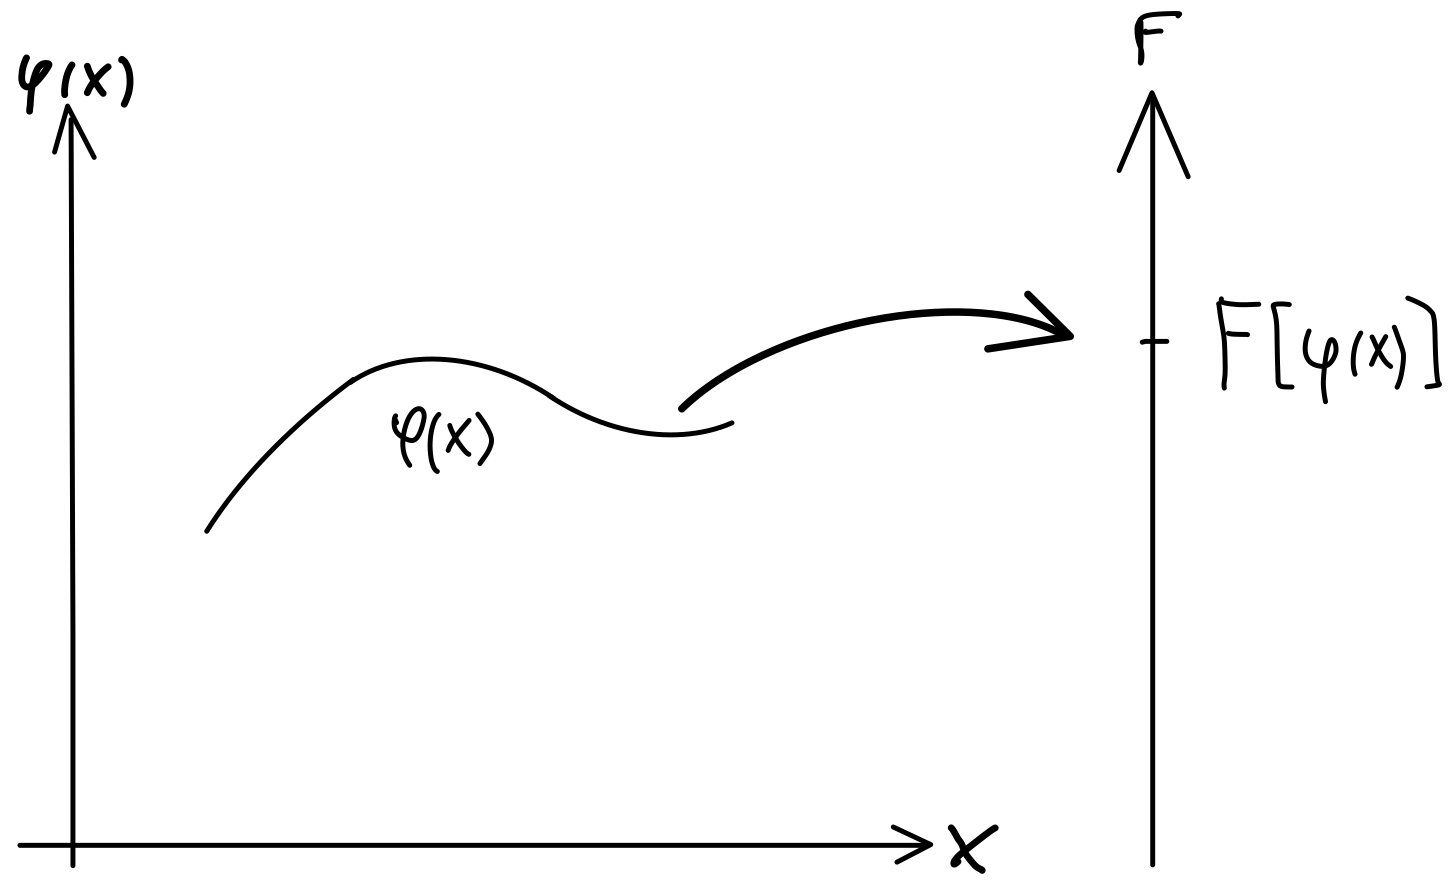
\includegraphics[width=0.4\textwidth]{fig/Funktional.png}
  \caption{Das Funktional der Funktion $\varphi(x)$. Man beachte, dass hiermit
  der gesamten Funktion $\varphi(x)$ ein Wert zugewiesen
  wird.\label{fig:functional}}
 \end{center}
\end{wrapfigure}
Gegeben eine Funktion $\varphi(x)$, dann nennen wir $F[\varphi(x)]$ ein
Funktional. Dies ist eine Erweiterung des Konzepts einer Funktion
$F(\varphi_1,\varphi_2,\dots)=F(\varphi_i)$ mehrerer Variabler, bei der wir den
diskreten Index $i$ durch eine kontinuierliche Variable $x$ ersetzen. Ein
Funktional ordnet also einer Funktion $\varphi(x)$ einen Wert zu. Wir stellen
uns das vor, wie in Abbildung \ref{fig:functional} skizziert.\\
\\
\\
\\
\\
\\
\\
\\
\\

\begin{example}{Verschiedene Beispiele von Funktionalen}
Ein Funktional kann repräsentiert sein durch
\begin{itemize}
\item 
$F[\varphi]=\int\limits_a^b\varphi(x)dx$, das Integral von $\varphi(x)$
  über einem Intervall $[a,b]$, oder
\item 
  $F[\varphi]=\int\limits_a^bf(\varphi(x))dx$, das Integral einer Funktion
  $f$ von $\varphi(x)$ auf dem Intervall $[a,b]$, oder
\item 
  $F[\varphi]=\int\limits_a^bf(\varphi(x), \varphi'(x))dx$, das Integral
  einer Funktion $f$ von $\varphi(x)$, die auch von der Ableitung $\varphi'(x)$
  abhängt, oder 
\item 
  $F[\varphi]=\varphi(y)=\int\limits_a^b\varphi(x)\delta(y-x)dx$, einem
  Integral dessen Integrand die Deltafunktion enthält, usw. 
\end{itemize}
  Eine Erweiterung auf mehrere Funktionen, die auch noch von mehreren Variablen
  abhängen können ist möglich $F[\varphi_i(x_k)]$. Dabei kann
  $F[\varphi_i(x_k)]$ auch ein Integral einer Funktion $f$ der $\varphi_i(x_k)$
  und deren partieller Ableitungen sein.
\end{example}
\section{Exkurs zur Diracschen Deltafunktion}\label{sec:Deltafunktion}
Zunächst sei hier eine Warnung ausgesprochen. Deltafunktionen sind keine
Funktionen im eigentlichem Sinne, obwohl sie oftmals so bezeichnet werden. In
der Mathematik werden diese Objekte als Distributionen bezeichnet. Da ihre
Wirkung auf echte Funktionen von ihrer genauen Definition abhängt, ist
Vorsicht bei ihrer Anwendung geboten.
\subsection{Definition der Deltafunktion}
Wir beginnen mit einem Beispiel und legen die Folge von Glockenkurven
\begin{equation}\label{eq:Lorentzian}
y(x,\varepsilon)=\frac{1}{\pi}\frac{\varepsilon}{x^2+\varepsilon^2}
\end{equation}
zugrunde. Mit kleiner werdendem $\varepsilon$ werden diese Funktionen immer
schmaler und höher, wie man in Abbildung \ref{fig:Glockenkurven} sehen kann.

Im Limes $\varepsilon\rightarrow 0$ ist die Funktion gleich Null für $x\ne 0$
und für $x=0$ divergiert sie. Wir schreiben dies formal als
\[ \lim_{\varepsilon\rightarrow 0} y(x,\varepsilon)=
  \left\{\begin{matrix}0& x\ne 0\\\infty& x=0\end{matrix}\right.\]
Die unter den in (\ref{eq:Lorentzian}) definierten Kurven liegende Fläche ist
\[\int_{-\infty}^{\infty}\frac{1}{\pi}\frac{\varepsilon}{x^2+\varepsilon^2}dx=
  \left.\frac{1}{\pi}\arctan \frac{x}{\varepsilon}\right|_{-\infty}^{\infty}=1.\]
Diese ist unabhängig von $\varepsilon$ immer 1, wie wir sehen.

\begin{wrapfigure}[18]{l}{0.45\textwidth}
  \begin{center}
   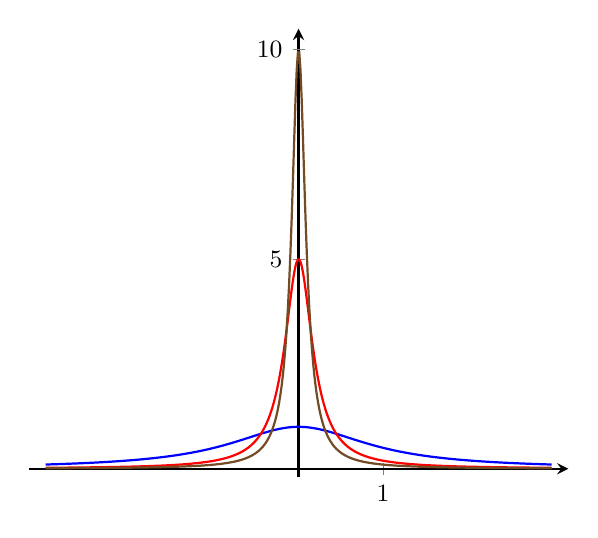
\begin{tikzpicture}%[domain=0:4]
    \begin{axis}[domain=-3:3,
	xmin=-3.2, xmax=3.2,
	ymin=-.2, ymax=10.5,
        axis y line=center,
        axis x line=middle,
	style = thick,
	xticklabel style = { font = \small, anchor = north},
	xtick = {1},
	ytick={\empty},
	extra y ticks= {5,10},
	extra y tick labels = {5,10},
	extra y tick style = { font = \small, anchor = west},
        samples=400]
      \addplot+[mark=none] {1./(x^2+1.)};
      \addplot+[mark=none] {.2/(x^2+.04)};
      \addplot+[mark=none] {.1/(x^2+.01)};
    \end{axis}
   \end{tikzpicture}
  \end{center}
  \caption{\label{fig:Glockenkurven}Glockenkurven wie in (\ref{eq:Lorentzian})
  definiert, mit den $\varepsilon$-Werten 1. (blau), 0.2 (rot) und 0.1 (grün).}
\end{wrapfigure}
Gegeben eine stetige Funktion $f(x)$. Wir betrachten das Integral
\[I(\varepsilon)=\int_{-\infty}^{\infty}f(x)y(x,\varepsilon)dx\]
als Funktion von $\varepsilon$ und schreiben den Grenzübergang formal als
\begin{equation}\label{eq:intfy}
  \lim_{\varepsilon\rightarrow 0}\int_{-\infty}^{\infty}f(x)y(x,\varepsilon)dx=
\int_{-\infty}^{\infty}f(x)\delta(x)dx
\end{equation}

Die so definierte Deltafunktion ist ein Symbol und keine Funktion im Sinne der
Analysis. Wir sollten uns stets vor Augen halten, dass die Bildung des
Grenzwertes $\lim_{\varepsilon\rightarrow 0}$ mit der Integration über $x$
nicht vertauschbar ist, das heißt, dass vor der Limesbildung stets die
Integration auszuführen ist.\vspace{1cm}

Um den Grenzwert in (\ref{eq:intfy}) ausrechnen zu können, machen wir die
Substitution $x=\varepsilon\xi$. Damit erhalten wir
\[ F(\varepsilon)=\int_{-\infty}^{\infty}f(\varepsilon\,\xi)
\frac{1}{\pi}\frac{1}{\xi^2+1}d\xi\]
Das Integral über die Glockenfunktion ist, wie wir bereits ausgerechnet haben,
gegeben als
\[\int_{-\infty}^{\infty}\frac{1}{\pi}\frac{1}{\xi^2+1}d\xi=1.\]
Damit können wir den Grenzübergang $\varepsilon\rightarrow 0$ in
$F(\varepsilon)$ unter dem Integral ausführen und erhalten
\[F(0)=\int_{-\infty}^{\infty}f(0)
\frac{1}{\pi}\frac{1}{\xi^2+1}d\xi=f(0)\]
\subsection{Eigenschaften der Deltafunktion}
Gegeben eine stetige Funktion $g(x)$ mit einfachen Nullstellen bei $x_n$, d.h.
$g(x_n)=0$ und $g'(x_n)\ne 0$, so gilt
\[\delta(g(x))=\sum\limits_n\frac{1}{|g'(x_n)|}\delta(x-x_n)\]

Bilden wir die Ableitung der Funktion $y(x,\varepsilon)$ nach $x$, so erhalten
wir von der Glockenkurve ausgehend 
\[y'(x,\varepsilon)=-\frac{2}{\pi}\frac{\varepsilon x}{(\varepsilon^2+x^2)^2}\]
Nun berechnen wir den Grenzübergang des Integrals
\begin{equation}\label{eq:deltaderivative}
\lim_{\varepsilon\rightarrow 0}\int_{-\infty}^{\infty}f(x)y'(x,\varepsilon)dx=
\underbrace{\left.\lim_{\varepsilon\rightarrow 0}f(x)y(x,\varepsilon)\right|_{-\infty}^{\infty}}_{0}
-\lim_{\varepsilon\rightarrow 0}\int_{-\infty}^{\infty}f'(x)\delta(x)dx
\end{equation}
In (\ref{eq:deltaderivative}) zeigt sich im ersten Term auf der rechten Seite
der Gleichung die erste Schwierigkeit. Damit dieser an den Grenzen
verschwindet, muss $y(x,\varepsilon)$ im Gernzübergang schneller gegen Null
gehen als $f(x)$. Daher die Warnung am Anfang des Abschnitts.

Wir erinnern uns an die Fourierintegrale (\ref{eq:fourierhin}, \ref{eq:fourierrueck})
\[
F(k)=\int_{-\infty}^{\infty}e^{-ikx}f(x)dx\\
f(x)=\frac{1}{2\pi}\int_{-\infty}^{\infty}e^{ikx}F(k)dk
\]
Setzen wir die erste in die zweite Zeile ein, dann erhalten wir
\[f(x)=\frac{1}{2\pi}\int_{-\infty}^{\infty}\int_{-\infty}^{\infty}e^{ik(x-x')}f(x')dx'dk\]
mit der Integration über $k$ nach der über $x'$. Wenn das Gleichheitszeichen
gelten soll, dann muss
\[\delta(x-x')="\frac{1}{2\pi}\int_{-\infty}^{\infty}e^{ik(x-x')}dk".\]
Wobei ``'' bedeutet, dass die Integration über $k$ erst nach der über $x'$
erfolgen soll. Dies ist die Fourierdarstellung der $\delta$-Funktion.
%
\section{Funktionalableitung oder Variation des Funktionals}\label{sec:Funktionalableitung}
Gegeben das Funktional $F[\varphi(x)]$. Wenn wir nun die Funktion $\varphi(x)$
um einen Wert $\Delta\varphi$ verändern , dann ändert
sich auch das Funktional
$F[\varphi+\Delta\varphi]=F[\varphi]+\Delta F$. 

Um dies zu verstehen, variieren wir $\varphi(x)$ nur in einer endlichen
Umgebung $dx_0$ des Punktes $x_0$, also
$F[\varphi+\varepsilon(x_0,dx_0)\Delta\varphi]$, mit 
  \begin{equation}\label{eq:umgebungeps}
    \varepsilon(x_0,dx_0)=\left\{\begin{matrix}1\text{ für
    }x\in[x_0-\frac{dx_0}{2},x_0+\frac{dx_0}{2}]\\ 0 \text{
    sonst}\end{matrix}\right.
  \end{equation}
Damit schreiben wir $\Delta F=F[\varphi +\varepsilon(x_0,dx_0) \Delta\varphi]
-F[\varphi]$. Dies schreiben wir im Grenzübergang für verschwindende
$\Delta\varphi$ und $dx_0$ als
\begin{equation}\label{eq:Variationsableitung}
  \lim_{dx_0\rightarrow 0}\lim_{\Delta\varphi\rightarrow 0}
      \frac{F[\varphi+\varepsilon(x_0,dx_0)\Delta\varphi]-F[\varphi]}{\Delta\varphi dx_0}
    =\frac{\delta F[\varphi]}{\delta\varphi(x_0)}
\end{equation} 
Diese Funktionalableitung oder Variation von $F$ ist die Varallgemeinerung der
partiellen Ableitung $\frac{\partial F[\vec{\varphi}]}{\partial\varphi_k}$.
%
\begin{figure}[!h] 
 \begin{center}
  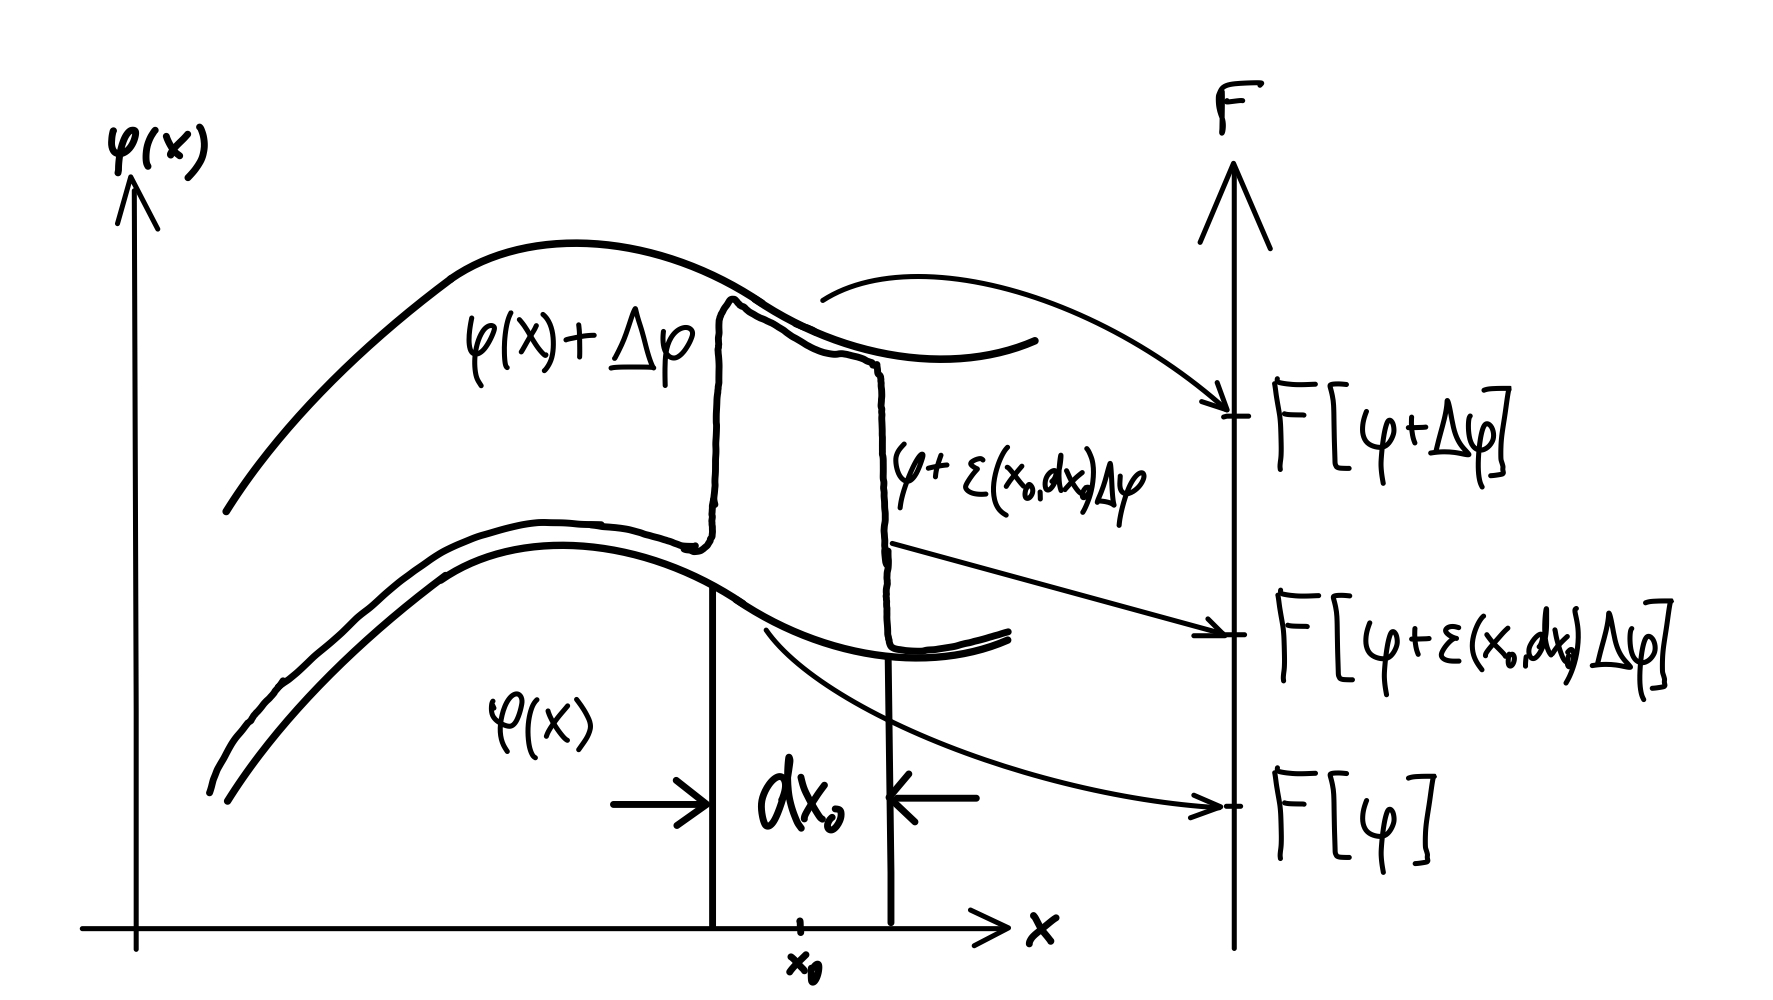
\includegraphics[height=0.4\textwidth]{fig/Variation.jpeg}
  \caption{Die Variation eines Funktionals der Funktion $\varphi(x)$. Wie
    ändert sich das Funktional, wenn die gesamte Funktion $\varphi(x)$ variiert
    wird? $F[\phi]$ ist der Wert den Funktionals,
    $F[\phi+\varepsilon(x_0,dx_0)\Delta\varphi]$ ist der Wert des Funktionals
    wenn wir in einer $\varepsilon$-Umgebung von $x_0$ die Funktion $\varphi$
    um $\Delta\varphi$ ändern. Somit ist die Änderung des Funktionals $\Delta
    F=F[\phi+\varepsilon(x_0,dx_0)\Delta\varphi]-F[\phi]$, wenn wir in einer
    $\varepsilon$-Umgebung von $x_0$ die Funktion $\varphi$ um $\Delta\varphi$
    ändern. Die gesamte Änderung ergibt sich nun durch das Integral über $\Delta
    F$.\label{fig:variation}}
 \end{center}
\end{figure}
%
Das Differential $\Delta F$ zu einer beliebigen differentiellen Veränderung
$\delta\varphi$ erhalten wir durch Integration über alle $x_0$
\begin{equation}\label{eq:DifferentialVariation}
  \Delta F = \int\frac{\delta F[\varphi]}{\delta\varphi(x_0)}\Delta\varphi(x_0)dx_0,
\end{equation}
wobei die entsprechende diskrete Version des Differentials, wie wir bereits
wissen, folgendermaßen definiert ist
\begin{equation}\label{eq:DifferentialMultiD}
    \Delta F = \sum\limits_k \frac{\partial F[\varphi_k]}{\partial\varphi_k}\Delta\varphi_k
\end{equation}
%
\subsection{Liste wichtiger Funktionalableitungen}\label{sec:WichtigeAbleitungen}
\begin{itemize}
  \item Sei $F[\varphi]=\varphi(\tilde{x})$ dann erhalten wir
    \[
      \frac{\delta\varphi(\tilde{x})}{\delta\varphi(x)}=\lim_{dx_0\rightarrow 0}\lim_{\Delta\varphi\rightarrow 0}
      \frac{\varphi(\tilde{x})+\varepsilon(\tilde{x},x,dx_0)\Delta\varphi-\varphi(\tilde{x})}{\Delta\varphi dx_0}=\lim_{dx_0\rightarrow 0}\frac{\varepsilon(\tilde{x},x,dx_0)}{dx_0}=\delta(\tilde{x}-x)
    \]
  \item Mit der obigen Überlegung und $F[\varphi]=\varphi'(\tilde{x})$ erhalten wir analog
    \[
      \frac{\delta\varphi'(\tilde{x})}{\delta\varphi(x)}=\frac{d}{d\tilde{x}} \frac{\delta\varphi(\tilde{x})}{\delta\varphi(x)}=\frac{d}{d\tilde{x}}\delta(\tilde{x}-x)=-\frac{d}{dx}\delta(\tilde{x}-x)
    \]
    wobei hier wieder Vorsicht geboten ist mit der Wirkung der Ableitung einer
    Deltafunktion (siehe Abschnitt \ref{sec:Deltafunktion}).
  \item Für $F[\varphi]=f(\varphi(\tilde{x}))$ erhalten wir mit Hilfe der Kettenregel
    \[
      \frac{\delta f(\varphi(\tilde{x}))}{\delta\varphi(x)}
      =\frac{df}{d\varphi}\frac{\delta \varphi(\tilde{x})}{\delta\varphi(x)}
      =\frac{df}{d\varphi}\delta(\tilde{x}-x).
    \]
    Deshalb haben wir im Fall  $F[\varphi]=f(\varphi(\tilde{x}),\varphi'(\tilde{x}))$
      \[
	\frac{\delta f(\varphi(\tilde{x}),\varphi'(\tilde{x}))}{\delta\varphi(x)}=
	\frac{\partial f(\varphi(\tilde{x}),\varphi'(\tilde{x})}{\partial\varphi(\tilde{x})}\delta(\tilde{x}-x)-
	  \frac{\partial f(\varphi(\tilde{x}),\varphi'(\tilde{x})}{\partial\varphi'(\tilde{x})}\frac{d}{dx}\delta(\tilde{x}-x).
    \]
  \item Setzen wir $F[\varphi]=\int f(\varphi(\tilde{x}))d\tilde{x}$ dann erhalten  wir 
    \[
      \frac{\delta F[\varphi]}{\delta\varphi(x)}=\int \frac{\partial f(\varphi(\tilde{x}))}{\partial\varphi(x)}d\tilde{x}=
      \int\frac{\partial f(\varphi(\tilde{x}))}{\partial\varphi(\tilde{x})}\frac{\partial\varphi(\tilde{x})}{\partial\varphi(x)}d\tilde{x}=
      \int\frac{\partial f(\varphi(\tilde{x}))}{\partial\varphi(\tilde{x})}\delta(\tilde{x}-x)d\tilde{x}=\frac{\partial f}{\partial\varphi}
    \]
\end{itemize}

Wir wenden die obigen Fälle auf das Funktional $F[\varphi]=\int
f(\varphi(\tilde{x}),\varphi'(\tilde{x}))d\tilde{x}$ an und erhalten
 \[
   \frac{\delta F[\varphi]}{\delta\varphi(x)}=\int \frac{\delta f(\varphi(\tilde{x}),\varphi'(\tilde{x}))}{\delta\varphi(x)}d\tilde{x}=
   \int\left(\frac{\partial f(\varphi(\tilde{x}),\varphi'(\tilde{x}))}{\partial\varphi(\tilde{x}))}\delta(\tilde{x}-x)-
 \frac{\partial f(\varphi(\tilde{x}),\varphi'(\tilde{x}))}{\partial\varphi'(\tilde{x})}\frac{d}{dx}\delta(\tilde{x}-x)\right)d\tilde{x}.
    \]
Die Ableitung nach „x“ unter dem Integral können wir vor das Produkt ziehen, so dass wir
\[
   \frac{\delta F[\varphi]}{\delta\varphi(x)}=\int \frac{\delta f(\varphi(\tilde{x}),\varphi'(\tilde{x}))}{\delta\varphi(x)}d\tilde{x}=
   \int\left(\frac{\partial f(\varphi(\tilde{x}),\varphi'(\tilde{x}))}{\partial\varphi(\tilde{x})}-\frac{d}{dx}
       \frac{\partial f(\varphi(\tilde{x}),\varphi'(\tilde{x}))}{\partial\varphi'(\tilde{x})}\right)\delta(\tilde{x}-x)d\tilde{x}.
\]
erhalten. Nach dem Ausführen der Integration bleibt
\[
  \frac{\delta F[\varphi]}{\delta\varphi(x)}=\frac{\partial f(\varphi(x),\varphi'(x))}{\partial\varphi(x)}
  -\frac{d}{dx} \frac{\partial f(\varphi(x),\varphi'(x))}{\partial\varphi'(x)}
\]
 Dies ist ein wichtiges Ergebnis, das wir im folgenden genauer betrachten
 wollen.
%
\subsection{Das Extremalprinzip in der Mechanik}
Gegeben sei eine Funktion $L(q(t),\dot q(t))$. Wir stellen uns die Frage für
welche Funktion $q(t)$ das Funktional
\[
  S[q(t)]=\int_a^b L(q(t),\dot q(t)) dt
\]
extremal wird. D.h. wir suchen unter allen möglichen Funktionen $q(t)$
diejenige, die $S[q(t)]$ extremal werden lässt. Oder in anderen Worten, wir
wollen dasjenige $q(t)$ finden, für das jegliche Variation von $S[q(t)]$
verschwindet, also 
\[\frac{\delta S[q]}{\delta q}=0\]
Diese Variation haben wir aber bereits im vorigen Abschnitt als Beispiel angegeben
\[
  \frac{\delta S[q]}{\delta q}=\frac{\partial L(q(t),\dot q(t)}{\partial q(t)}
    -\frac{d}{dt} \frac{\partial L(q(t),\dot q(t))}{\partial \dot q(t)}=0
\]
\begin{note}{Der harmonische Oszillator}
Wir setzen $L(q(t),\dot q(t))=\frac{1}{2}m\dot
q(t)^2-\frac{1}{2}k q(t)^2$ und erhalten
\[ \frac{\partial L(q(t),\dot q(t)}{\partial q(t)}
    -\frac{d}{dt} \frac{\partial L(q(t),\dot q(t))}{\partial \dot q(t)}=
   -kq(t)-\frac{d}{dt}m\dot q(t)
   =0.
 \]
 Dies ist die wohlbekannte Bewegungsgleichung des harmonischen Oszillators\newline 
 \[m\ddot q(t)+kq(t)=0.\]

Hieraus folgern wir, ohne dass wir hier den Beweis antreten, dass die
Lagrangefunktion $L=T^*-V$ eines mechanischen Systems aus der Differenz
zwischen kinetischer 
Koenergie\footnote{Die Unterscheidung zwischen kinetischer Energie
  $T=\frac{p^2}{2m}$ und kinetischer Koenergie $T^* =\frac{mv^2}{2}$ ist nur
  wichtig im Falle, dass der Impuls nicht mehr als $p=m\cdot v$ geschrieben
  werden kann. Dies ist z.B. der Fall, wenn relativistische Effekte wichtig
  werden. Wir nehmen an, dass dies im Folgenden nicht der Fall sei und machen
  fortan diese Unterscheidung nicht.}
%
$T^*$ und potentieller Energie V gebildet wird. Indem wir fordern, dass die
Variation des Integrals über die Lagrangefunktion verschwindet, erhalten wir
die Bewergungsgleichungen, der entsprechenden mechanischen Systeme. Diese
Gleichungen nennen wir die Euler-Lagrange-Gleichungen.
\end{note}
Wir fügen ein Beispiel allgemeinerer Natur an.
\begin{example}{Das Brachistochronenproblem}
  \begin{wrapfigure}{l}{0.5\textwidth}
  \centering
  \begin{tikzpicture}[scale=0.8]
    \begin{axis}[domain=0:4.0, xmin=0, xmax=3.8, ymin=0, ymax=5, axis y line = left,
     axis x line = bottom, axis line style = {-latex}, 
     xticklabel style = { font = \small, anchor = north}, xtick = {\empty}, ytick = {\empty},
     xlabel style={at={(rel axis cs:1.05,.15)}}, xlabel=$x$,
     ylabel style={at={(rel axis cs:0.2,1.05)},rotate=-90}, ylabel=$y$,
     extra x ticks = {3.8},
     extra x tick labels = {$x_0$},
     extra y ticks = {4.5},
     extra y tick labels = {$y_0$},
     extra y tick style = { font = \small, anchor = west},
     samples=400]
     \addplot+[mark=none] {4.5*((x-3.8)^2)/14.44};
     \addplot+[mark=none] {4.5*((x-3.8)^2)/14.44+0.2*sin(x*47.37)-.2*sin(3*x*47.37)-.15*sin(4*x*47.37)};
    \end{axis}
   \end{tikzpicture}
   \caption{Verschiedene Notrutschen.}
  \label{fig:Rutsche}
 \end{wrapfigure}
  Unsere Aufgabe sei es, eine Notrutsche für die Evakuierung eines Flugzeugs zu
  konstruieren. Die Rutsche soll eine solche Form haben, dass die Passagiere
  darauf auf dem schnellsten Weg den Boden erreichen.  Die Situation ist in
  \ref{fig:Rutsche} schematisch dargestellt. Die Passagiere steigen bei $x=0$
  auf die Rutsche in einer Höhe von $y=y_0$ und rutschen zum Punkt $x=x_0$ bei
  $y=0$.

  Hier ist eine Funktion $y(x)$ gesucht, die eine Bedingung erfüllen muss, die
  wir nun formulieren wollen. Wir gehen von Energieerhaltung aus, d.h. die
  Lageenergie am Einstiegspunkt wird bis zum momentanen Punkt auf der Rutsche
  in kinetische Energie umgewandelt, oder 
  \[ mgy_0=\frac{1}{2}m(\dot{y}^2+\dot{x}^2)+mgy \]
  oder
  \begin{equation}
  g(y_0-y)=\frac{1}{2}\left[\left(\frac{dx}{dt}\right)^2
    +\left(\frac{dy}{dt}\right)^2\right]
    \label{eq:Rutschenergie}
  \end{equation}
  Wie wir sehen, kürzt sich die Masse raus. D.h. schwere und leichte Passagiere
 rutschen gleich schnell. Ist das Modell vollständig?
 
 Wir schreiben (\ref{eq:Rutschenergie}) um
 \begin{equation}
   (dt)^2=\frac{(dx)^2+(dy)^2}{2g(y_0-y)}
   \label{eq:RutscheAufgeloest}
 \end{equation}
 (\ref{eq:RutscheAufgeloest}) kann nun benutzt werden um die Zeit $T$ zu berechnen,
 die es braucht um auf einer gegebenen Funktion $y(x)$ von $(0,y_0)$ nach
 $(x_0,0)$ zu rutschen. Die Zeit $T$ ist ein Funktional
 \begin{equation}
    T[y]=\int\limits_{0}^{x_0}\sqrt{\frac{1+\left(\frac{dy}{dx}\right)^2}{2g(y_0-y)}}dx
    =\int\limits_{0}^{x_0}\sqrt{\frac{1+y'(x)}{2g(y_0-y(x))}}dx
    =\int\limits_{0}^{x_0}f(y(x),y'(x))dx=F[y]
   \label{eq:Zeitfunktional}
 \end{equation}
 Damit haben wir das Variationsproblem $\frac{\delta T[y]}{\delta y}=0$ zu
 lösen. D.h. bei welchem $y$ ist $T$ minimal? Aus der obigen Liste der
 wichtigsten Funktionalableitungen in Abschnitt \ref{sec:WichtigeAbleitungen}
 sehen wir, dass wir die Euler-Lagrange Gleichungen
 \[ 
   \frac{\partial f(y(x),y'(x))}{\partial y(x)}
    -\frac{d}{dx} \frac{\partial f(y(x),y'(x)}{\partial y'(x)}=0
 \]
 benutzen können und bekommen damit eine Differentialgleichung zur Bestimmung
 von $y(x)$.
\end{example}
%
\subsection{Variation von Mehrfachintegralen}
Wir erweitern den Begriff des Funktionals, wie wir ihn in Abschnitt
\ref{sec:DasFunktional} definierten, indem wir anstatt des Integrals der
Funktion $L(q(t),\dot q(t))$ nun ein Funktional betrachten, das aus einem
Mehrfachintegral besteht. Dafür setzen wir anstatt der Funktion $q(t)$, das
Feld $\varphi(x_{\mu})$ in $L$ ein und schreiben die Funktion $L$ von nun an
als $\mathcal{L}$. Hierbei bezeichne $x_{\mu}$ die $\mu$-te unabhängige
Variable. Ausserdem erweitern wir die in $\mathcal{L}$ vorhandenen Ableitungen
auf die partiellen Ableitungen erster und höherer Ordnung der Funktion
$\varphi(\mathbf{x})$. Damit ist $\mathcal{L}$ eine Funktion 
\begin{equation}\label{eq:LagrangeDensity}
  \mathcal{L}=\mathcal{L}\left(\varphi(x_\mu),\frac{\partial\varphi(x_\mu)}{\partial x_{\nu}},
  \frac{\partial^2\varphi(x_\mu)}{\partial x_{\nu}\partial x_{\kappa}}\dots ;\, x_\mu\right)
\end{equation}
und wir haben ein mehrdimensionales Variationsproblem vorliegen. Das Funktional
sei gegeben als n-dimensionales Integral
\begin{equation}\label{eq:nDFunktional}
  J[\varphi]=\int\limits_{\Omega}\mathcal{L}\left(
    \varphi(x_\mu),\partial_{\nu}\varphi(x_\mu),
    \partial_{\nu\kappa}\varphi(x_\mu)\dots ;\, x_\mu\right)d^nx_\mu
\end{equation}
wobei wir für $\frac{\partial}{\partial x_{\nu}}=\partial_{\nu}$,
$\frac{\partial^2}{\partial x_{\mu}\partial x_{\nu}} =\partial_{\mu\nu}$
geschrieben haben. Variieren wir nun die Funktion $\varphi(x_\mu)$ um einen
Wert $\psi(x_\mu)$, wie bereits in Abschnitt \ref{sec:Funktionalableitung}
beschrieben, dann erhalten wir für die Variation des Integrals in
(\ref{eq:nDFunktional})
\begin{align} \label{eq:VariationFeld}
  \delta J[\varphi]=& J[\varphi+\varepsilon\psi]-J[\varphi]=\\
  =&\int\limits_{\Omega}\Bigl[\mathcal{L}(
    \varphi(x_\mu)+\varepsilon\psi(x_\mu),
      \partial_{\nu}\varphi(x_\mu)+\varepsilon\partial_{\nu}\psi(x_\mu),
      \partial_{\nu\kappa}\varphi(x_\mu)+\varepsilon\partial_{\nu\kappa}\psi(x_\mu)\dots ;\, x_\mu)\nonumber\\
      &-\mathcal{L}( \varphi(x_\mu),\partial_{\nu}\varphi(x_\mu),
     \partial_{\nu\kappa}\varphi(x_\mu)\dots ;\, x_\mu)\Bigr]d^n x_\mu \nonumber
\end{align}
Wir entwickeln (\ref{eq:VariationFeld}) in eine Potenzreihe nach $\varepsilon$
und behalten alle Glieder bis zur ersten Ordnung, dann erhalten wir
\begin{equation}\label{eq:VariationTaylor1}
  \delta J[\varphi]=\varepsilon\int\limits_{\Omega}\Bigl(
    \frac{\partial\mathcal{L}}{\partial\varphi}\psi
    +\frac{\partial\mathcal{L}}{\partial(\partial_{\mu}\varphi)}\partial_{\mu}\psi
  +\frac{\partial\mathcal{L}}{\partial(\partial_{\mu\nu}\varphi)}\partial_{\mu\nu}\psi+\cdots\Bigr)d^n x_\mu
\end{equation}
Wir wählen $\psi$ dergestalt, dass es auf dem Rand des Integrationsgebietes
verschwindet, also $\psi(x_{\mu}\in\Omega)=0$, dann erhalten wir durch
partielle Inegration von (\ref{eq:VariationTaylor1})
\begin{equation}\label{eq:VariationFunktionalFeld}
 \delta J[\varphi]=\varepsilon\int\limits_{\Omega}\left(
    \frac{\partial\mathcal{L}}{\partial\varphi}
    -\partial_{\mu}\frac{\partial\mathcal{L}}{\partial(\partial_{\mu}\varphi)}
    +\partial_{\mu\nu}\frac{\partial\mathcal{L}}{\partial(\partial_{\mu\nu}\varphi)}
  -\cdots\right)\psi\, d^n x_\mu
\end{equation}
Für beliebige $\psi$ folgen daraus die Bewegungsgleichungen für das Feld $\varphi(x_\mu)$ zu
\begin{equation}
  \frac{\partial\mathcal{L}}{\partial\varphi}
  -\partial_{\mu}\frac{\partial\mathcal{L}}{\partial(\partial_{\mu}\varphi)}
  +\partial_{\mu\nu}\frac{\partial\mathcal{L}}{\partial(\partial_{\mu\nu}\varphi)}
  -\partial_{\mu\nu\gamma}\frac{\partial\mathcal{L}}{\partial(\partial_{\mu\nu\gamma}\varphi)}
  \cdots=0
  \label{eq:EulerLagrangeFeld}
\end{equation}
\subsection{Die schwingende Saite, ein ausführliches Beispiel}
\begin{tikzpicture} %[domain=0:4]
    \begin{axis}[%width=\textwidth,height=0.5\textwidth, 
	width=16cm,
	height=8cm,
        hide x axis,
        hide y axis,
        samples=400]
	\addplot+[domain=0:180,mark=none,ultra thick] {(cos(x))};
	\draw[thick,decoration={aspect=0.41, segment length=2.3mm, 
	amplitude=2.2mm,coil},decorate] (0.0,200.0) -- (0.0,100.0);
	\node at (10,150) {$k$};
	\node at (170,50) {$k$};
	\draw[thick,decoration={aspect=0.41, segment length=2.3mm, 
	amplitude=2.2mm,coil},decorate] (180,0.0) -- (180,100.0);
	\draw[-Latex,thick] (-10,-20) -- (-10,200);
	\node[above] at (-10,200) {u};
	\draw[-Latex,thick] (-10,100) -- (190,100);
	\node[right] at (190,100) {x};
	\draw[thick, dashed] (0,100) -- (0,200);
	\draw[thick, dashed] (180,0) -- (180,100);
	\node at (10,80) {$x=0$};
	\node at (170,120) {$x=\ell$};
	\draw[thick] (130,100) -- (130,95);
	\draw[thick] (150,100) -- (150,95);
	\node [above] at (140,40) {$\Delta x$};
	\node [right] at (150,25) {$\Delta u$};
	\node [left] at (145,15) {$\sqrt{\Delta x^2+\Delta u^2}=\Delta s$};
	\addplot+[domain=130:150,mark=none,ultra thick] {(cos(130))};
	\addplot[color=red,mark=none,ultra thick] coordinates { (150,{cos(130)}) (150,{cos(150)}) };
	\addplot[color=red,mark=none,ultra thick] coordinates { (130,{cos(130)}) (150,{cos(150)}) };
    \end{axis}
   \end{tikzpicture}

Eine Seite der Länge $\ell$ sei bei $x=0$ und $x=\ell$ jeweils über eine Feder
elastisch aufgehängt. Die Aufhängepunkte sollen sich nur senkrecht zur
x-Richtung bewegen können (siehe Zeichung). Die Saite habe eine Massendichte
$\rho$ pro Längeneinheit und eine Spannung $\tau$. Die Federn der Aufhängung
haben eine Fedekonstante $k$.
   
Die kinetische Energie eines Abschnitts $\Delta x$ der Saite ist 
\[
  \Delta T^*=\frac{1}{2}\Delta m\cdot v^2 =
  \frac{1}{2}\rho\Delta x\left(\frac{\partial
  u(x,t)}{\partial t}\right)^2,
\] 
wobei wir kleine Relativauslenkungen $\Delta u$ angenommen haben. Die gesamte
kinetische Energie ist die Summer aller Beiträge der Abschnitte $\Delta x$. Im
Grenzübergang $\Delta x\rightarrow 0$ wird hieraus ein Integral 
\begin{equation}\label{eq:Ekin}
  T^*=\frac{1}{2}\rho\int_0^\ell\left(\frac{\partial
  U(x,t)}{\partial t}\right)^2dx
\end{equation}

Dasselbe machen wir nun mit der potentiellen Energie. Aus der Grafik erkennen
wir, dass die elastische Energie gleich der Saitenspannung $\tau$ multipliziert
mit der Steckung $\Delta x$ ist. Ohne auslenkung können wir so die gesamte
elastische Energie ausrechnen. Wenn aber lokal eine Verschiebung $\Delta u$
vorliegt, dann wir die Saite gedehn auf die neue Länge $\sqrt{\Delta x^2+\Delta
u^2}=\Delta s$. Die elastische Energie, die die Saite zusätlich durch die
Dehnung aufnimmt ist gerade die Differenz $\Delta V=\tau\cdot(\sqrt{\Delta
x^2+\Delta u^2}-\Delta x)$. Dies können wir auch schreiben als $\Delta
V=\tau\cdot\left(\sqrt{1+\left(\frac{\Delta u}{\Delta
x}\right)^2}-1\right)\Delta x$. Für klein Dehnungen $\left(\frac{\Delta u}{\Delta
x}\right)$ entwickeln wir den Term unter der Wurzel und erhalten näherungsweise
\[
  V=\tau\cdot\left(1+\left(\frac{\Delta u}{\Delta x}\right)^2-1\right)\Delta x
  =\tau\cdot\left(\frac{\Delta u}{\Delta x}\right)^2\Delta x
\]
Im Grenzübergang wird hieraus
\begin{equation}
  V=\frac{1}{2}\tau\int_0^\ell\left(\frac{\partial u}{\partial x}\right)^2dx.
  \label{eq:Epot}
\end{equation}
Wir müssen noch die zwei potentiellen Energieterme an den Aufhängepunkten
berücksichtigen, diese sind
\begin{equation}
  V_k=\frac{1}{2}k\cdot u(0,t)^2 +\frac{1}{2}k\cdot u(\ell,t)^2.
  \label{eq:EpotSprings}
\end{equation}
Damit erhalten wir folgende Lagrangefunktion
\begin{equation}
  L=\int_0^\ell\left[
    \frac{\rho}{2}\left(\frac{\partial u(x,t)}{\partial t}\right)^2
   -\frac{\tau}{2}\left(\frac{\partial u(x,t)}{\partial x}\right)^2
 \right]dx-\frac{1}{2}k\left(u(0,t)^2 + u(\ell,t)^2\right).
  \label{eq:LagrangianSaite}
\end{equation}

Das Funktional $J[u]=\int_{t_0}^{t_1}L(u(x,t))dt$ nennen wir das
Wirkungsintegral. Wir berechnen die Variation des Wirkungsintegrals
\begin{flalign}\label{eq:VariationAction}
  \delta &J[u]=J[u+\varepsilon\psi]-J[u]\\
  &=\varepsilon\int_{t_0}^{t_1}\left\{\int_0^\ell\left[
    \rho\frac{\partial u(x,t)}{\partial t}\frac{\partial\psi(x,t)}{\partial t}
  -\tau\frac{\partial u(x,t)}{\partial x}\frac{\partial\psi(x,t)}{\partial x}
   \right]dx
 - k\left[u(0,t)\psi(0,t)+u(\ell,t)\psi(\ell,t)\right]\right\}dt\nonumber\\
  &=\varepsilon\int_{t_0}^{t_1}\int_0^\ell\left[
    -\rho\frac{\partial^2u(x,t)}{\partial t^2}
 +\tau\frac{\partial^2u(x,t)}{\partial x^2}\right]\psi(x,t)dxdt
 -\varepsilon\int_0^\ell k\left[u(0,t)\psi(0,t)+u(\ell,t)\psi(\ell,t)\right]dt\nonumber\\
 &+\varepsilon\int_{t_0}^{t_1}\tau\left[\frac{\partial u(\ell,t)}{\partial x}\psi(\ell,t)-
 \frac{\partial u(0,t)}{\partial x}\psi(0,t)\right]dt
 +\varepsilon\int_0^\ell\rho\left[\frac{\partial u(x,t_0)}{\partial t}\psi(x,t_0)-
   \frac{\partial u(x,t)}{\partial t}\psi(x,t_1)\right]dx\nonumber
\end{flalign}
Assume that for $t=t_0$ and $t=t_1$ we do not vary the path $u$, so the last
term in (\ref{eq:VariationAction}) vanishes and therefore we get to first order
in $\varepsilon$
\begin{align}\label{eq:VariationActionFinal}
\delta &J[u]=\varepsilon\int_{t_0}^{t_1}\int_0^\ell\left[
    -\rho\frac{\partial^2u(x,t)}{\partial t^2}
 +\tau\frac{\partial^2u(x,t)}{\partial x^2}\right]\psi(x,t)dxdt\nonumber\\
 &-\int_{t_0}^{t_1}\left(\tau\frac{\partial u(0,t)}{\partial x}+ku(0,t)\right)\psi(0,t)dt
 -\int_{t_0}^{t_1}\left(-\tau\frac{\partial u(\ell,t)}{\partial x}+ku(\ell,t)\right)\psi(\ell,t)dt
\end{align}
$J[u]$ nimmt ein Extermum an, wenn $\delta J[u]=0$ gilt und zwar für beliebige
Variationen $\psi(x,t)$ des Pfades $u(x,t)$. Also setzen wir zunächst einmal
eine Variation mit $\psi(0,t)=\psi(\ell,t)=0$ an. Dies führt auf die Bewegungsgleichung
\begin{equation}
   -\rho\frac{\partial^2u(x,t)}{\partial t^2}
 +\tau\frac{\partial^2u(x,t)}{\partial x^2}=0
  \label{eq:MotionString}
\end{equation}
Wenn $u(x,t)$ (\ref{eq:MotionString}) genügt, dann ist der erste Term in
(\ref{eq:VariationActionFinal}) immer null. Setzen wir abwechselnd
$\psi(0,t)=0$ und $\psi(\ell,t)\ne 0$ und umgekehrt, dann erhalten wir zwei
zusätzliche Gleichungen
\begin{align}
  \tau\frac{\partial u(0,t)}{\partial x}+ku(0,t)&=0\label{eq:BCStringLeft}\\
  \tau\frac{\partial u(\ell,t)}{\partial x}+ku(\ell,t)&=0\label{eq:BCStringRight}
\end{align}
(\ref{eq:BCStringLeft}) und (\ref{eq:BCStringRight}) sind die zu
(\ref{eq:MotionString}) gehörigen Randbedingungen. Diese Beispiel zeigt, wie
mit Hilfe der Variationsrechnung die Bewegungsgleichungen für ein System
ageleitet werden kann.